\documentclass[thesis.tex]{subfiles}

\begin{document}

\chapter{Original ATACCC analysis} \label{ATACCC:sec:original-analysis}

This appendix describes an early analysis I did on an initial version of the ATACCC dataset.
This dataset is not publicly available.
It contains 79 individuals, all those in the study at that time with at least one positive test.
The duration distribution estimated is very similar to that in \cref{E-ATACCC} but more certain because it assumes that the random effects are drawn independently.

\section{Methods}

\subsection{Model of viral load}

For an individual $i$, their trajectory is determined by two points and one slope parameter.
The points are the time at which the individual has a 50\% chance of testing positive, $t_{i,0}$, and the time at which their viral load
peaks, $t_{i,\text{peak}}$ after $t_{i,0}$; the slope parameter, $\beta_i$ determines the rate their Ct increases (viral load decreases) following the peak.
The Ct value for an individual at time $t_{i,0}$ is the known limit of detection, $C_\text{lod}$,
Their Ct value at the peak is $C_{i,\text{peak}}$ and inferred.
The slope parameter, $\beta_i$, determines how quickly an individual's Ct value increases following the peak viral load.
We denote the vector of the parameters defined here as $\vec\theta_i = \begin{bmatrix} t_{i,0} & t_{i,\text{peak}} & C_{i,\text{peak}} &  \beta_i \end{bmatrix}^T$.

This parameterization leads to the following Ct value trajectory for individual $i$:
$$
\hat{C}_i(t, \vec\theta_i) = \begin{cases}
  C_{\text{lod}} + (C_{i,\text{peak}} - C_{\text{lod}}) \frac{t - t_{i,0}}{t_{i,\text{peak}}}
    &t \leq t_{i,\text{peak}} + t_{i,0} \\
  C_{i,\text{peak}} + \beta_i (t - t_{i,\text{peak}} - t_{i,0})
    &t > t_{i,\text{peak}} + t_{i,0}.
\end{cases}
$$

Day 0 for an individual is the day they were enrolled in the study and first swabbed.

\subsection{Observation model and likelihood}

Observed Ct values are assumed to be drawn from a normal distribution with mean $\hat{C}_i(t)$ and standard deviation $\sigma_\text{obs}$.
censored at the limit of detection.
Additionally, we introduce a probability of a false negative $\eta$, to account for negative test results seen near the peak viral load.
Denoting an observed Ct value for individual $i$ at time $t$ as $y_{i,t}$ with
$y_{i,t} = \infty$ for a negative test, this gives the following likelihood.
$$
\pi(y_{i,t} \mid \vec\theta_i, \sigma_\text{obs}, \eta) = \begin{cases}
  (1 - \eta) f_N(y_{i,t} \mid \hat{C}_i(t, \vec\theta_i), \sigma_\text{obs}^2) &y_{i,t} < \infty \\
  \eta + (1 - \eta) (1 - F_N(C_\text{lod} \mid \hat{C}_i(t, \vec\theta_i), \sigma_\text{obs}^2)) & y_{i,t} = \infty
\end{cases}
$$
where $\sigma_\text{obs}$ is a model parameter determining the variability in
test results, and $f_N(y \mid \mu, \sigma^2)$ and $F_N(y \mid \mu, \sigma^2)$ are the pdf
and cdf (respectively) of a normal distribution with mean $\mu$ and variance $\sigma^2$.

We assume that all observations (both of the same and different individuals) are independent conditional on the model parameters.
The parameter $\vec\theta_i$ introduces dependence between observations of the same individuals.
\Cref{sec:paper:hierarchy} explains the hierarchical structure which borrows information between individuals.

\subsection{Hierarchical structure}\label{sec:paper:hierarchy}

We assume that $\log t_{i,\text{peak}}$, $C_{i,\text{peak}}$, and $\log \beta_i$ are drawn independently from univariate normal distributions (details below).
Other parameters are not hierarchical and have prior distributions placed on them in the normal way; \cref{fig:paper:model_DAG} shows these relationships.
As in \textcite{fogartyBayesian}, a log transform is applied to the parameters which must be positive for biological plausibility.
As well as restricting these parameters to be positive, this enables the skewed distribution observed in SARS-CoV-2 with some individuals testing positive for much longer than the median.

The formal specification of this, including the required population-level parameters is:
\begin{align}
    \log t_{i,\text{peak}} &\dist N(\mu_{\log t_\text{peak}}, \sigma_{\log t_\text{peak}}^2) 
    \label{eq:paper:tpeak}\\
    C_{i,\text{peak}} &\dist N(\mu_{C_\text{peak}}, \sigma_{C_\text{peak}}^2) 
    \label{eq:paper:Cpeak}\\
    \log \beta_i &\dist N(\mu_{\log \beta}, \sigma_{\log \beta}^2).
    \label{eq:paper:beta}
\end{align}

\begin{figure}
    \centering
    \makebox[\textwidth][c]{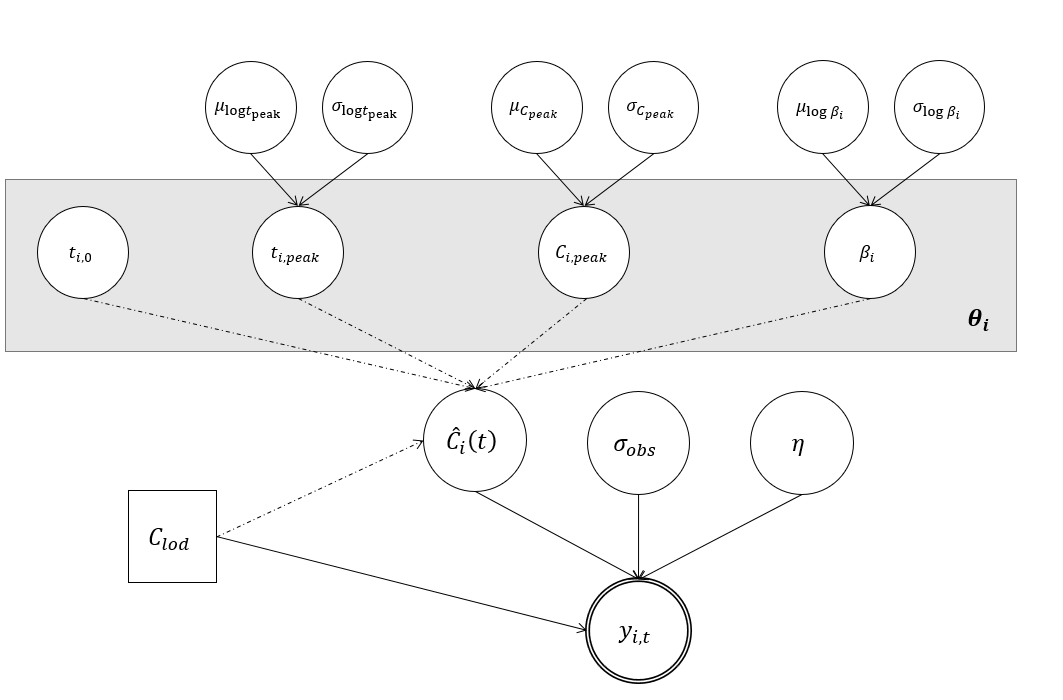
\includegraphics[scale=0.8]{ATACCC/appendix/Bayesian_piecewise_DAG}}
    \caption[DAG showing hiearchical structure]{Directed acyclic graph showing the relationship between parameters in the model. Dotted lines represent deterministic (functional) relationships and solid lines stochastic (distributional) relationships. The box represents a fixed (known) quantity and double circle an observed quantity (the data). Index $i$ ranges over individuals, and $t$ over time. Parameters indexed by $i$ exist once for each individual. See main text for equations governing the relationships and the distributions used.}
    \label{fig:paper:model_DAG}
\end{figure}

\subsection{Inference}

Inference was performed by Hamiltonian Monte Carlo (HMC) implemented in Stan 2.26.1~\autocite{Stan-2-32-2}.
To aid with mixing, the hierarchical parameters were implemented using the non-centred parameterization~\autocites{papaspiliopoulosGeneral,stanReparameterization}.
In addition, $t_{i,0}$ was reparameterized in terms of the absolute time of peak.
Convergence was assessed by checking R-hat < 1.1, and visual inspection of traceplots, and effective sample size.

\subsection{Priors}

Weakly informative priors were used on all parameters except $\mu_{\log t_\text{peak}}$ and $\sigma_{\log t_\text{peak}}$.
The latter were chosen to reflect the prior belief that viral load peaks shortly before symptom onset, which occurs a median of 5.1 days after infection~\autocite{mcaloonIncubation}.

\begin{table}[ht]
\centering
\begin{tabular}{llrrr}
  \hline
    Parameter & Distribution & 0.05 & 0.5 & 0.95 \\ 
  \hline
    $\eta$ & $\text{Beta}(0.95, 9)$ & $0$ & $0.07$ & $0.28$ \\ 
    $\sigma_\text{obs}$ & $\text{Half-Cauchy}(0, 0.67)$ & $0.05$ & $0.67$ & $8.51$ \\ 
    $t_{0,i}$ & $N(0, 5^2)$ & $-8.22$ & $0$ & $8.22$ \\ 
    $\mu_{\log t_\text{peak}}$ & $N(\log(3), \log(2.5)^2)$ & $\log (0.66)$ & $\log (3)$ & $\log (13.54)$ \\ 
    $\sigma_{\log t_\text{peak}}$ & $\text{Half-Cauchy}(0, 0.67)$ & $0.05$ & $0.67$ & $8.51$ \\ 
    $\mu_{C_\text{peak}}$ & $N(17, 5^2)$ & $8.78$ & $17$ & $25.22$ \\ 
    $\sigma_{C_\text{peak}}$ & $\text{Half-Cauchy}(0, 4)$ & $0.31$ & $4$ & $50.82$ \\ 
    $\mu_{\log\beta}$ & $N(\log(3.5), \log(1.4)^2)$ & $\log (2.01)$ & $\log (3.5)$ & $\log (6.09)$ \\ 
    $\sigma_{\log\beta}$ & $\text{Half-Cauchy}(0, 0.67)$ & $0.05$ & $0.67$ & $8.51$ \\
   \hline
\end{tabular}
\caption[Priors]{Priors used, columns 3 to 5 gives quantiles of the distributions specified. See main text for description of the parameters.}
\label{tab:paper:priors}
\end{table}

\section{Results}

\subsection{Goodness of fit}

The model generally shows a good fit to the observed data (see \cref{fig:paper:goodness_of_fit}).
For individuals with few or no observations before their peak viral load, information is borrowed from other individuals to infer when this is likely to have occurred.
Most observations, excluding those that look to be false negatives (negatives surrounded by two high viral load positives) fall within the 95\% predictive intervals.

\begin{figure}
    \centering
    \vspace*{-3cm}
    \makebox[\textwidth][c]{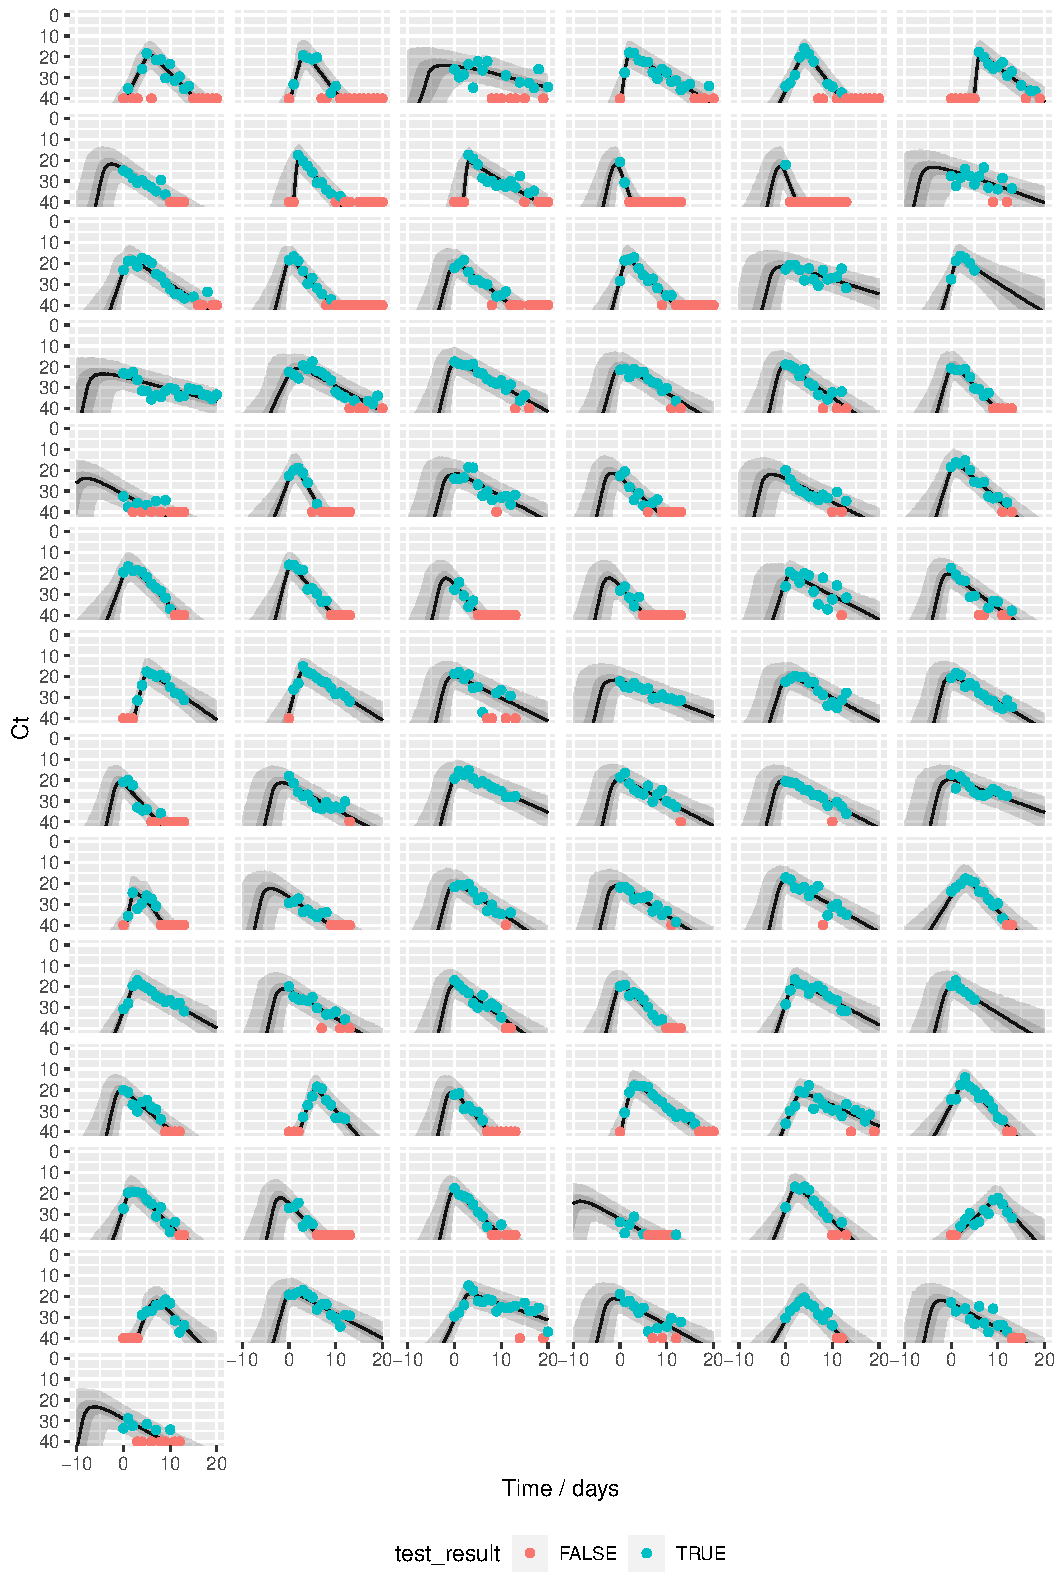
\includegraphics[scale=0.9]{ATACCC/appendix/goodness_of_fit}}
    \caption[Goodness-of-fit]{Predictive median (solid line), 50\% and 95\% predictive intervals (light and dark shading respectively) for test results (ignoring false negatives). Points show actual observations.}
    \label{fig:paper:goodness_of_fit}
\end{figure}

\subsection{Parameter estimates}

We estimate that the time from when an individual has a 50\% chance of detection to peak viral load (equivalently: when $\hat{C} = C_\text{lod}$) is 2.4 (posterior median; with 95\% central CrI 1.5--3.3) days with a population standard deviation on the log scale of 0.69 (0.42--1.06).
The mean peak viral corresponds to 17.8 (17.1--18.6) Ct units, with a standard deviation of 2.2 (1.5--3.2) Ct units, after which the decrease in viral corresponds to Ct values increasing by 1.6 (1.5--1.8) Ct / day, with a standard deviation on the log scale of 0.50 (0.40--0.61).
Predictive distributions for these parameters for a new individual are shown in \cref{fig:paper:indiv_predict}.
We estimate a 6.8 (5.0--8.8) \% probability of a false negative independent of the viral load of an individual.

\begin{figure}
    \centering
    \makebox[\textwidth][c]{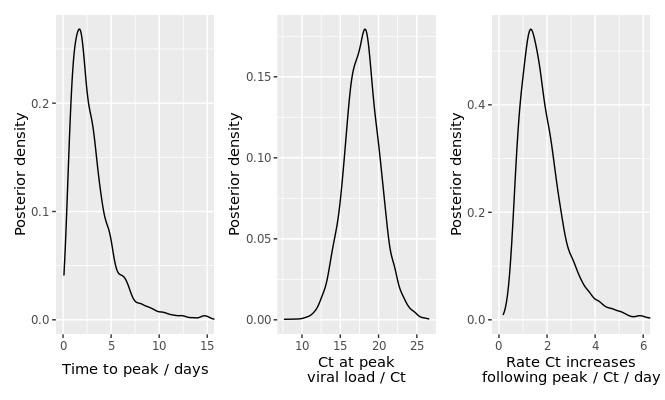
\includegraphics{ATACCC/appendix/indiv_predictive}}
    \caption{Posterior predictions of model parameters for a new, previously unobserved individual.}
    \label{fig:paper:indiv_predict}
\end{figure}

The time between the two points when $\hat{C} = C_\text{lod}$ for an individual can be considered a duration of infection.
This gives a mean duration estimated at 18.4 (16.5--20.9) days but the distribution is skewed, as seen by the median of 16.6 (14.8--18.5) days.
The full distribution is in \cref{fig:paper:duration}.
\begin{figure}
    \centering
    \makebox[\textwidth][c]{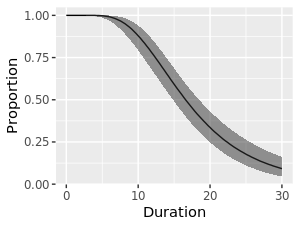
\includegraphics{ATACCC/appendix/duration}}
    \caption[Proportion of population positive]{Proportion of people with $\hat{C} > C_\text{lod}$ a given number of days after this first occurred. Shading indicates central 95\% credible interval.}
    \label{fig:paper:duration}
\end{figure}

\section{Discussion}

This study presents estimates of viral load dynamics based on a general population sample with daily swabbing.
Our results show a peak Ct value around 5 Ct lower than \textcite{kisslerViral}, that is a higher viral load, although occurring at a similar time (see \cref{tab:paper:compare}) and a longer time from first detection to peak viral load than \textcite{jonesEstimating}.
This could be because of the different populations in each study. \Textcite{kisslerViral}'s data is collected from longitudinal swabbing of individuals professionally involved in the National Basketball Association (NBA).
Of the individuals who were included in their analysis, around half were in professional athletes, likely in peak physical condition, and 90\% were male.
Our data is collected from the general population who were reported as contacts of individuals detected through surveillance open to all members of the public.
Therefore, our sample is likely to be, on average, in worse physical condition which may lead to a higher viral load (lower Ct).
Another possible difference could be the lab the tests were performed in.
Ct values are not fully comparable between different laboratories due to different testing methodologies~\autocites{dahdouhCt,hanRTPCR}.

Our estimate for the duration of detectable infection, 18.4 (16.5--20.9) days, is similar to a recent meta-analysis~\autocite{cevikShedding}.
However, since individuals were tested for a maximum of 21 days in this study, a large part of the distribution is extrapolated.

\begin{table}[]
    \centering
    \makebox[\textwidth][c]{\begin{tabular}{p{7cm}ccc}
    Quantity & This study & \Textcite{kisslerViral} \\ 
    \hline
    Mean time from first detectable to peak viral load / days & 2.4 (1.5--3.3) & 3.2 (2.4--4.2) \\
    Mean Ct at peak viral load / Ct & 17.8 (17.1--18.6) & 22.4 (20.7--24.0) \\
    Mean increase in Ct following peak / Ct / day & 1.6 (1.5--1.8) & 2.1 (1.7--2.6)
    \end{tabular}}
    \caption[Comparison to previous studies.]{Summary of results in comparison to previous studies. \Textcite{jonesEstimating} do not give values in terms of Ct.}
    \label{tab:paper:compare}
\end{table}


\end{document}